\section{Methodology}  
\label{Sec:Methodology}

\subsection{System Pipeline}

Figure~\ref{fig:exp_pipeline} illustrates the full evaluation pipeline. For each task, \oursys provides a unified description including function interface, reference implementation, and task-specific constraints. Each method generates a candidate kernel through its dedicated adapter. All kernels are then evaluated by the same pipeline, with intermediate logs retained for error analysis.

\begin{figure*}[t]
    \centering
    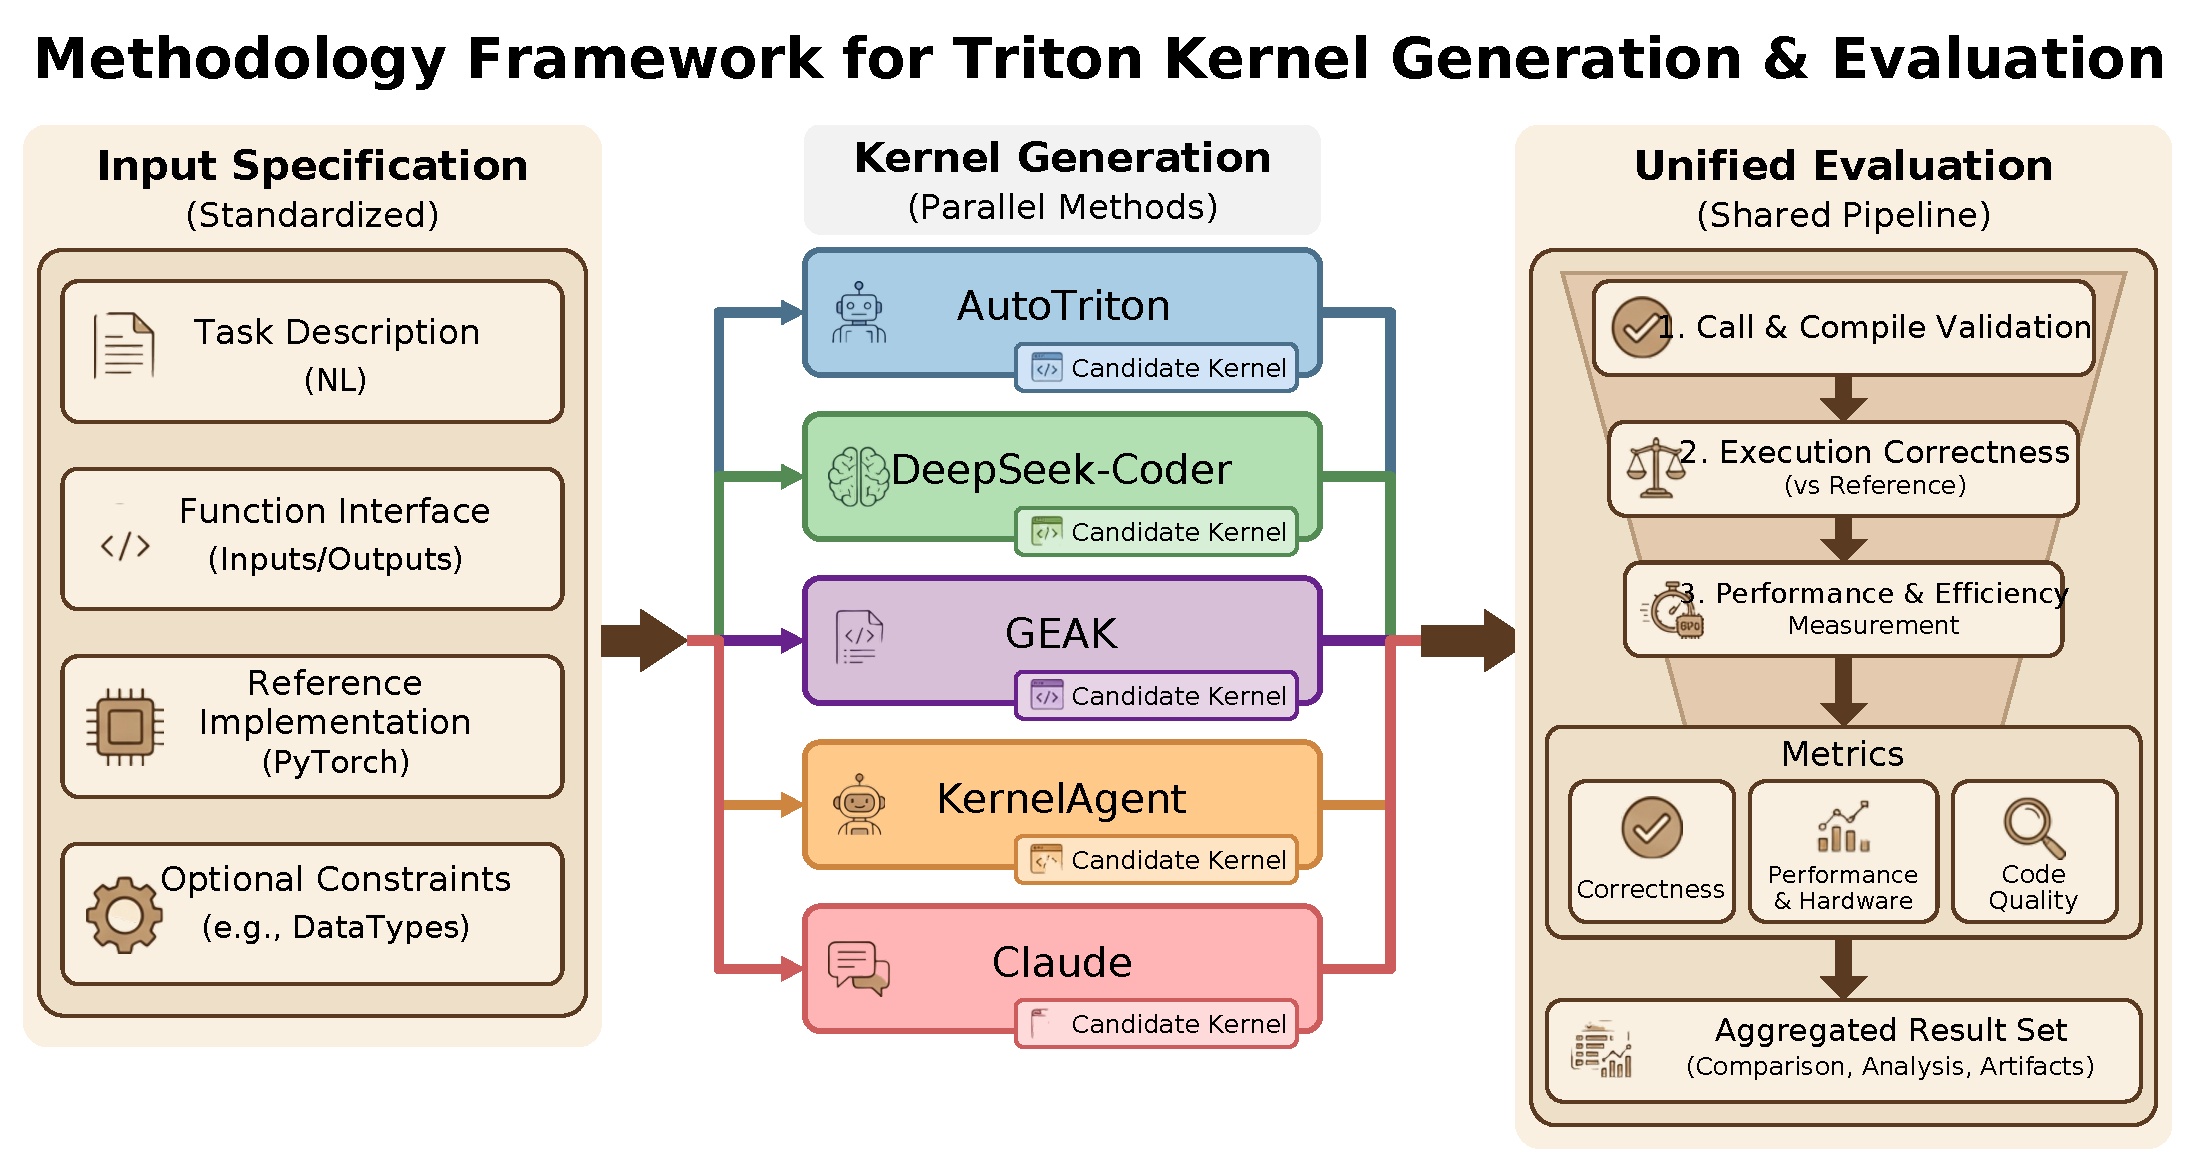
\includegraphics[width=\textwidth]{src/figs/exp_pipeline.pdf}
    \caption{Multiple methods generate Triton kernels from a shared task specification, and are evaluated under a unified pipeline measuring correctness, efficiency, and code quality.}
    \label{fig:exp_pipeline}
\end{figure*}

\subsection{Benchmark Design}

\subsubsection{Task Organization}

\oursys contains 176 tasks across 15 categories: Activation, Convolution, Fusion, Index, LinearAlgebra, Loss, Math, MatrixMultiply, Normalization, Optimizer, Pooling, Quantization, Random, Reduce, and SpatialOps. Categories were assigned based on computational structure rather than operator type, enabling comparison of tasks with similar parallel execution requirements.

The benchmark includes two main coverage extensions beyond TritonBench-T. First, selected fp16, bf16, and int8 multi-precision variants test whether methods can generate kernels under low-precision constraints. Second, six quantization tasks in W8A8 and W4A16 settings test whether methods can implement manual quantization logic—including scale computation, explicit casting, and dequantization—without relying on high-level APIs.

\subsubsection{Correctness Protocol}

\oursys uses a two-stage correctness protocol designed to reject implementations that pass simple output comparisons by chance.

\textbf{Call Accuracy} checks whether generated code can be imported, compiled, and called correctly, and whether it satisfies task-level constraints. For quantization tasks, a static checker additionally rejects forbidden high-level quantization APIs and verifies the presence of manual quantization logic including scale computation and explicit casting operations.

\textbf{Execution Accuracy} checks whether outputs match the reference implementation across multiple input distributions. Each task is evaluated under two modes: a standard mode sampling inputs from $\mathcal{N}(0,1)$, and an outlier mode injecting amplified outliers (probability 0.1\%, scale factor 50) to expose implementations that pass on typical inputs but fail under distributional shift. For standard tasks, dtype-aware numerical tolerances are applied. For quantization tasks, three metrics must simultaneously satisfy task-specific thresholds: cosine similarity ($\geq 0.90$--$0.95$), L1 relative error ($\leq 0.05$--$0.10$), and RMSE ($\leq 0.10$--$0.15$).


\subsubsection{Performance and Code Quality Protocol}

Runtime is measured with triton.testing.do\_bench (25 warmup, 100 measurement runs, median reported). Speedup is computed against the PyTorch eager baseline.
Hardware efficiency is measured as $\max(\mathrm{IOU}, \mathrm{MFU})$ to evaluate each kernel against its dominant bottleneck. Code quality is assessed through Maintainability Index (MI) and Cyclomatic Complexity (CC).

Note that FLOP- and byte-based quantities are derived from a fixed task-level target model (the intended computation under an idealized implementation), and should be interpreted as normalized efficiency proxies rather than measurements of the actual executed instructions.